% Q18 -- Scan-chain implementation: scannable flip-flops separated by logic clouds.
% Primary Inputs + Scan-In on the left; Flop1 -> Logic Cloud -> Flop2 -> Logic Cloud ->
% Flop3 -> Primary Outputs / Scan-Out; dashed scan chain links Flop1->Flop2->Flop3; CLK and
% SCAN control at the bottom.
\documentclass[border=10pt]{standalone}
\usepackage{tikz}
\usetikzlibrary{arrows.meta,positioning,shapes.geometric}
\begin{document}
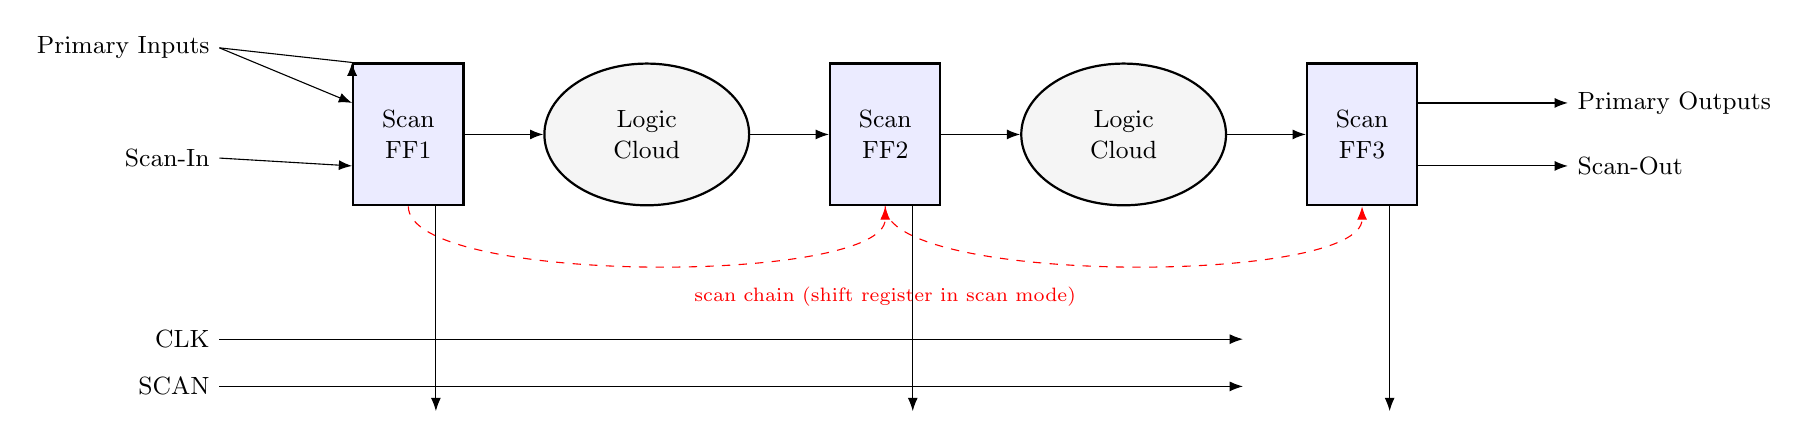
\begin{tikzpicture}[>=Latex, font=\small,
  ff/.style={draw, thick, fill=blue!8, minimum width=1.4cm, minimum height=1.8cm, align=center},
  cl/.style={draw, thick, fill=gray!8, ellipse, minimum width=2.6cm, minimum height=1.8cm, align=center}]
\node[ff] (f1) {Scan\\FF1};
\node[cl, right=1.0cm of f1] (c1) {Logic\\Cloud};
\node[ff, right=1.0cm of c1] (f2) {Scan\\FF2};
\node[cl, right=1.0cm of f2] (c2) {Logic\\Cloud};
\node[ff, right=1.0cm of c2] (f3) {Scan\\FF3};
% datapath
\draw[->] (f1) -- (c1); \draw[->] (c1) -- (f2);
\draw[->] (f2) -- (c2); \draw[->] (c2) -- (f3);
% primary inputs / scan-in
\draw[->] (-2.4,1.1) node[left]{Primary Inputs} -- (f1.north west) ++(0,0);
\draw[->] (-2.4,1.1) -- ([yshift=0.4cm]f1.west);
\draw[->] (-2.4,-0.3) node[left]{Scan-In} -- ([yshift=-0.4cm]f1.west);
% primary outputs / scan-out
\draw[->] ([yshift=0.4cm]f3.east) -- ++(1.9,0) node[right]{Primary Outputs};
\draw[->] ([yshift=-0.4cm]f3.east) -- ++(1.9,0) node[right]{Scan-Out};
% dashed scan chain linking the flops
\draw[->, dashed, red] (f1.south) .. controls +(0,-1) and +(0,-1) .. (f2.south);
\draw[->, dashed, red] (f2.south) .. controls +(0,-1) and +(0,-1) .. (f3.south);
\node[red, font=\scriptsize] at (f2.south)[below=0.9cm] {scan chain (shift register in scan mode)};
% control signals
\draw[->] (-2.4,-2.6) node[left]{CLK} -- (10.6,-2.6);
\draw[->] (-2.4,-3.2) node[left]{SCAN} -- (10.6,-3.2);
\foreach \n in {f1,f2,f3}{
  \draw[->] (\n.south) ++(0.35,0) -- ++(0,-2.6+0) ;
}
\end{tikzpicture}
\end{document}
